%% SECTION HEADER /////////////////////////////////////////////////////////////////////////////////////
\section{Damage indices}
\label{sec:di}

%% SECTION CONTENT ////////////////////////////////////////////////////////////////////////////////////
In the dissertation, six damage indices, considered to be the most effective \cite{torkamani2014novel, moix2016damage}, are analysed based on the signal envelope in the time-domain registered by the sensor.
All of them are considered in three options: (i) the full-length of the signal, (ii) the first wave packet of the \ac{s0}, (iii) the first wave packet of the \ac{a0}.
The analysis will consider signals at 50, 100 and 150 \unit{\kHz}, with the last frequency excluded for the \ac{a0}, because, as indicated in section~\ref{sec:resuls_pzt}, this mode is masked by reflections of the \ac{s0}.
The wave packets are extracted by windowing the full-length signals with a flattened Gaussian window in the form:
\begin{eqnarray}
	g(t)= \mathrm{exp}\left(-\left(\frac{t-t_0}{w_g}\right) ^{n}\right),
	\label{eq:psi_g}
\end{eqnarray}
\nomtypeD[gt]{\(g(t)\)}{Gaussian window}{}%
where \(t_0\) and \(w_g=0.5N_c/f_c\) are the center point and the half-width of the window, respectively, and  \(n\) determines the slope of the window.
The usage of the window is pictured in Fig.~\ref{fig:windows}.
\begin{figure}[!tbh]
	\begin{center}
		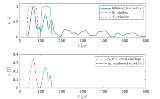
\includegraphics[width=0.95\textwidth]{Chapter_7/windows}
	\end{center}
	\caption{Signal envelop and Gaussian windows}
	\label{fig:windows}
\end{figure}


The following time-domain indices are taken into consideration: \ac{p2p}, \ac{saps}, \ac{sapr}, \acf{rmsd}, \ac{eng} and \ac{cc}.
Definitions of these metrics are given below:

\begin{eqnarray}
	\mathrm{P2P} & = & \left(\mathrm{max}(e_H) - \mathrm{max}(e_D)\right)\\
	\mathrm{SAPS} & = & 1 - \left(\frac{\mathrm{max}(e_H)-\mathrm{max}(e_D)}{\mathrm{max}(e_H)}\right)^2,\\
	\mathrm{SAPR} & = & \frac{\mathrm{max}(e_H)}{\mathrm{max}(e_D)},\\
	\mathrm{RMSD} & = & 1 - \sqrt{\frac{\sum_{i=1}^{n}\left[e_D-e_H\right]^2}	{\sum_{i=1}^{n}e_H^2}},\\
	\mathrm{ENG} & = & 1 -  \frac{\sum_{i=1}^{n}{e_D^2}-\sum_{i=1}^{n}{e_H^2}}{\sum_{i=1}^{n}{e_H^2}},\\
	\mathrm{CC} & = & \frac{n\sum_{i=1}^{n}e_De_H-\sum_{i=1}^{n}e_D\sum_{i=1}^{n}e_H}{\sqrt{n\sum_{i=1}^{n}e_D^2-\left[\sum_{i=1}^{n}e_D\right]^2}\sqrt{n\sum_{i=1}^{n}e_H^2-\left[\sum_{i=1}^{n}e_H\right]^2}},
\end{eqnarray}
where \(e_H\) and \(e_D\) are the envelope of the signal registered by the sensor for the healthy and damaged state of the sample, respectively, and \(n\) is the length of the signal.
The \ac{p2p}, \ac{saps}, \ac{sapr}  are based on the difference between amplitudes of the monitored and the baseline state.
The \ac{rmsd} measures the error between baseline and damaged, \ac{eng} compares the difference of the sensor responses energy and \ac{cc} is the index based on Pearson correlation coefficient.

\begin{figure}[!tbh]
	\begin{center}
		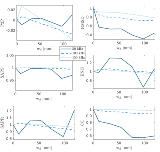
\includegraphics[width=0.95\textwidth]{Chapter_7/DI_full_full}
	\end{center}
	\caption{The \acfp{di} obtained with the \acf{fcgm} based on full-length signals.}
	\label{fig:DI_full_full}
\end{figure}
\begin{figure}[!tbh]
	\begin{center}
		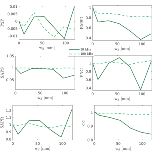
\includegraphics[width=0.95\textwidth]{Chapter_7/DI_full_A0}
	\end{center}
	\caption{The \acfp{di} obtained with the \acf{fcgm} based on \acs{a0} windowed signal.}
	\label{fig:DI_full_A0}
\end{figure}
\begin{figure}[!tbh]
	\begin{center}
		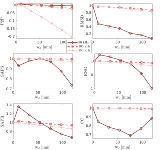
\includegraphics[width=0.95\textwidth]{Chapter_7/DI_full_S0}
	\end{center}
	\caption{The \acfp{di} obtained with the \acf{fcgm} based on \acs{s0} windowed signal.}
	\label{fig:DI_full_S0}
\end{figure}

The \acp{di} based on full-length signals derived from simulations with the \ac{fcgm} are presented in Fig.~\ref{fig:DI_full_full}.
The damage was modelled by removing the core cells in the damage area.
It can be noticed, all the \acp{di} for 50 \unit{\kHz} are not monotonous.
This is due to the fact that a low-frequency wave, according to work of Tian et al. \cite{tian2015wavenumber} up to 100 \unit{\kHz}, propagates through the entire thickness of the \ac{hsc}.
Therefore, in the analysis of damage size, not only the phenomenon of wave leakage is relevant, but also the reflection from cell walls.  
The high-frequency wave propagates mainly through the skin of the panel, so changes in the signal recorded by the sensor in the damaged sample are mainly caused by the wave leakage effect.

The \acp{di} based on the windowed signals are shown in Fig.~\ref{fig:DI_full_A0} and Fig.~\ref{fig:DI_full_S0} for the \ac{a0} and \ac{s0} window, respectively.
It should be mentioned that \acp{di} for 150 \unit{\kHz} are omitted in Fig.~\ref{fig:DI_full_A0}, due to the masking of this mode by the \ac{s0} reflections.
The characteristics of the indices are consistent with the related indices determined for the full-length signals.
However, the values of most windowed signals are lower than those of the full-length signals.
In addition, the \ac{s0} window-based \acp{di} have lower values than the \ac{a0} windowed signals, except the \ac{rmsd} at 50 \unit{kHz}.
It is because dominant displacements of the \ac{s0} are in-plane of the skin, so a smaller portion of the energy of the wave leak into the core through the healthy region.
In the case of the full-length response, the \ac{a0} is registered, which dominant displacements are out of the plate, making this mode more sensitive for damage in the form of disbonds or delamination.

Accordingly, the following indicators are chosen for further consideration: \ac{p2p} and \ac{sapr} at 150 \unit{kHz} (see Fig. \ref{fig:DI_P2P} and Fig. \ref{fig:DI_SAPR}), \ac{rmsd} and \ac{cc}, all in the case of full-length and at 100 and 150 \unit{\kHz} (see Fig. \ref{fig:DI_RMSD_full} and Fig. \ref{fig:DI_CC}), and \ac{rmsd} at 50 \unit{kHz} based on \ac{s0} windowed signals (see Fig. \ref{fig:DI_RMSD_S0}).
Those indices are compered with the \acp{di} obtained with the damage modelled by removing the interface elements and the results from simulations based on the \ac{hcgm} with both damage models.

\begin{figure}[!tbh]
	\begin{center}
		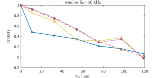
\includegraphics[width=0.95\textwidth]{Chapter_7/DI_P2P}
	\end{center}
	\caption{Comparison of the chosen \acfp{p2p} based on full-length signals for the various models of the core and damage: solid line the \acf{fcgm} with removed core cells, dashed line the \acf{fcgm} with removed interface elements, dash-dot line the \acf{hcgm} with removed core cells, dotted line the \acf{hcgm} with removed interface elements.}
	\label{fig:DI_P2P}
\end{figure}

\begin{figure}[!tbh]
	\begin{center}
		\includegraphics[width=0.95\textwidth]{Chapter_7/DI_SAPR}
	\end{center}
	\caption{Comparison of the chosen \acfp{sapr} based on full-length signals for the various models of the core and damage: solid line the \acf{fcgm} with removed core cells, dashed line the \acf{fcgm} with removed interface elements, dash-dot line the \acf{hcgm} with removed core cells, dotted line the \acf{hcgm} with removed interface elements.}
	\label{fig:DI_SAPR}
\end{figure}
It can be noticed that \ac{p2p} and \ac{sapr} differ significantly in terms of the core model used. Both indexes for the \ac{fcgm} are continuously decreasing, while for the \ac{hcgm}, the values are almost constant in the whole range of damage.
In addition, the damage model has little effect only for the \ac{fcgm}.

\begin{figure}[!tbh]
	\begin{center}
		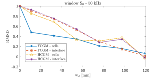
\includegraphics[width=0.95\textwidth]{Chapter_7/DI_RMSD_S0}
	\end{center}
	\caption{Comparison of the chosen \acfp{rmsd} based on \ac{s0} windowed signals for the various models of the core and damage: solid line the \acf{fcgm} with removed core cells, dashed line the \acf{fcgm} with removed interface elements, dash-dot line the \acf{hcgm} with removed core cells, dotted line the \acf{hcgm} with removed interface elements.}
	\label{fig:DI_RMSD_S0}
\end{figure}

The values for all cases are consistent for the \ac{rmsd} based on the \ac{s0} window.
Only the \ac{fcgm} for the two most minor damages deviates from the other models.
\begin{figure}[!tbh]
	\begin{center}
		\includegraphics[width=0.95\textwidth]{Chapter_7/DI_RMSD_full}
	\end{center}
	\caption{Comparison of the chosen \acfp{rmsd} based on full-length signals for the various models of the core and damage: solid line the \acf{fcgm} with removed core cells, dashed line the \acf{fcgm} with removed interface elements, dash-dot line the \acf{hcgm} with removed core cells, dotted line the \acf{hcgm} with removed interface elements.}
	\label{fig:DI_RMSD_full}
\end{figure}

\begin{figure}[!tbh]
	\begin{center}
		\includegraphics[width=0.95\textwidth]{Chapter_7/DI_CC_full}
	\end{center}
	\caption{Comparison of the chosen \acfp{cc} based on full-length signals for the various models of the core and damage: solid line the \acf{fcgm} with removed core cells, dashed line the \acf{fcgm} with removed interface elements, dash-dot line the \acf{hcgm} with removed core cells, dotted line the \acf{hcgm} with removed interface elements.}
	\label{fig:DI_CC}
\end{figure}

For the \ac{rmsd} and \ac{cc} based on full-length signals, the results are comparable for the all models, except the values for the \ac{hcgm} at 100 \unit{kHz} are more significant than the \ac{fcgm}.
